\section{Co-registered and geocoded MLC (CMLC \& GMLC)}
\label{sec:cmlc}

\subsection{Evaluation criteria}
\label{sec:cmlc_criteria}

We are proposing here to assess the performance of the phase products in two ways, i.e. by analyzing
\begin{itemize}
    \item The relative performance with real data by comparing with other phase estimators applied to the same data,
    \item The absolute performance by evaluating the algorithms on synthetic data.
\end{itemize}
In the second case, we are also going to develop a theoretical model to describe the coherence of interferograms which are generated internally by the progressive phase estimation algorithm.

The first approach has the advantage of situating the performance of the new algorithm with respect to known alternatives. It works on real data and thus maximizes the relevance for real-life applications.

The second approach has the advantage of checking the absolute performance and the behavior for specific, possibly critical, scenarios which might not be represented by the real-data dataset available for the study.

A more complete validation of the product would require further high-level processing to obtain deformation time series, which could then be compared to other products and sensors, like EGMS (European Ground Motion Service) or GNSS series. To do this in a proper way, one should also include atmospheric corrections, especially tropospheric ones. 
Despite the increased effort, a validation of this kind is going to have some limitations too: the differences between the sensors are going to result in different levels of noise, both on single measurements and on the mean velocity.
The activity should be understood more in terms of cross-comparison than pure validation.

This effort is, however, not necessary if we want to verify the core phase-estimation part, which is anyway the most critical and innovative contribution introduced in this project. Once the phase is well estimated, subsequent processing can follow the traditional PS/DS approach, including phase unwrapping and atmospheric corrections, which is well understood and validated.

\subsection{Relative performance assessment (SAOCOM)}
The algorithm for the generation of the MLC product is described in ATBD, let us call it progressive interferometric phase estimation (PIPE). In the plots, we are indicating it simply with "cmlc". The auto-regressive parameter for the running reference is chosen to be 0.95, whereas the long-term reference is a fixed snapshot of the running reference taken at the 10th acquisition.

We are going to discuss its performance with respect to
\begin{enumerate}
    \item EMI, a full-covariance phase estimation method (\cite{Ansari2018}),
    \item direct interferograms (indicated with "direct" in the plots),
    \item a version of progressive estimation without drift control and with fast-fading memory (indicated with "ndc", i.e. "no drift control", in the plots), to show a degraded performance.
\end{enumerate}


\begin{figure}[ht]
    \centering
    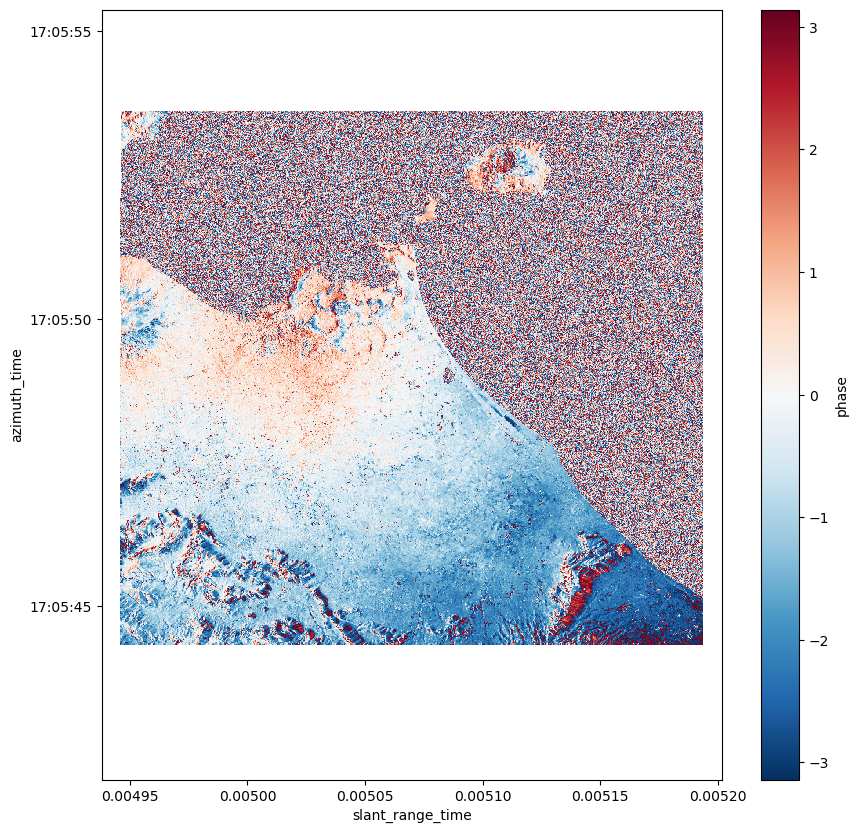
\includegraphics[width=0.45\linewidth]{Figures/mlc/DSC_S4/2025-01-14_2015-01-30_pipe.png}
    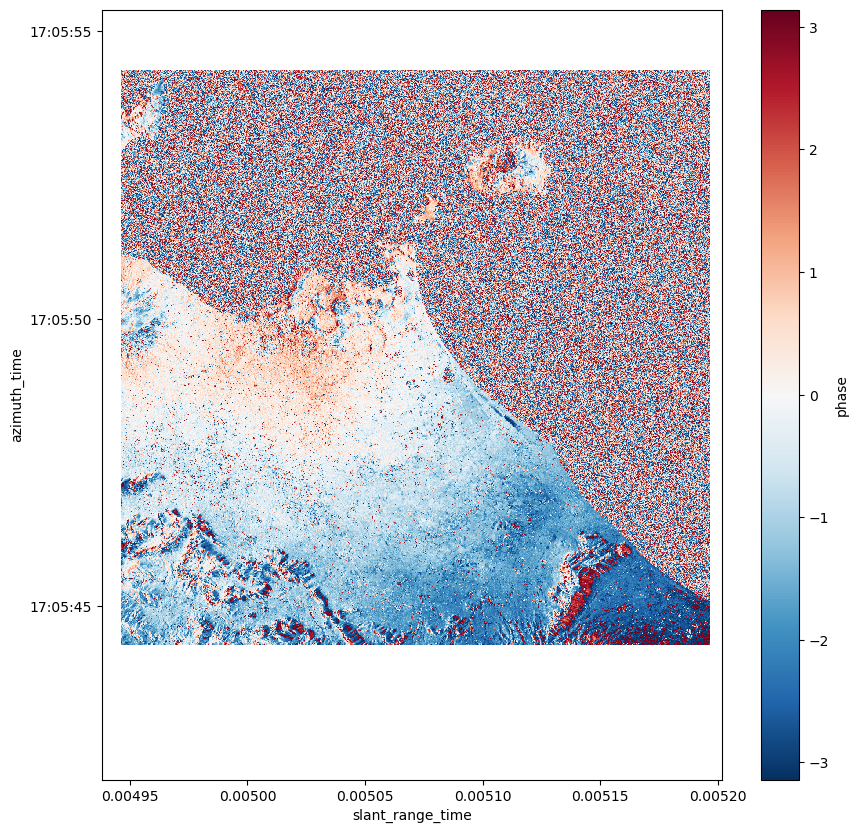
\includegraphics[width=0.45\linewidth]{Figures/mlc/DSC_S4/2025-01-14_2015-01-30_emi.png}
        \caption{The interferometric phase for the pair 2025-01-14 / 2025-01-30. Left: from the progressive interferometric phase estimation, right: from the EMI (full-covariance) estimation.}
    \label{fig:interf_pipe_emi}
\end{figure}

\begin{figure}[htb!]
    \centering
    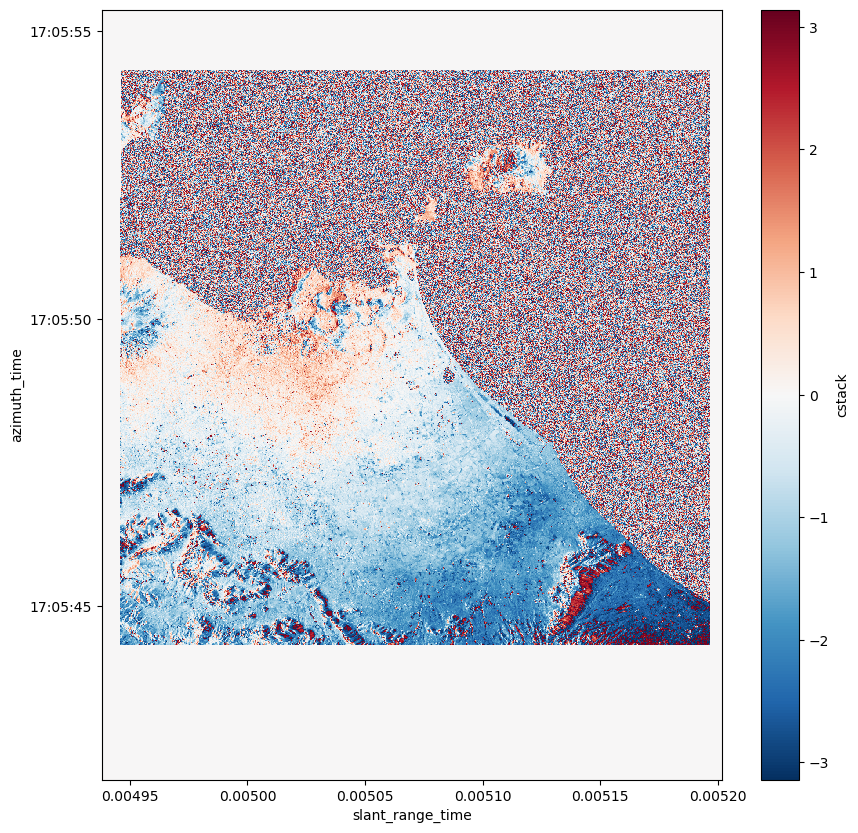
\includegraphics[width=0.45\linewidth]{Figures/mlc/DSC_S4/2025-01-14_2015-01-30_direct.png}
    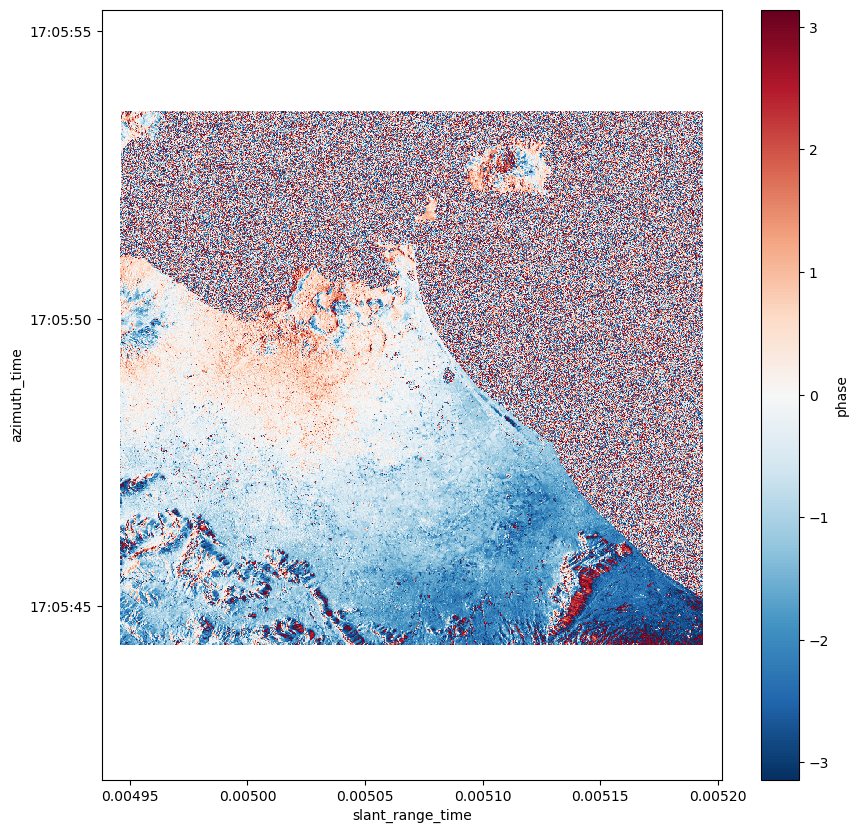
\includegraphics[width=0.45\linewidth]{Figures/mlc/DSC_S4/2025-01-14_2015-01-30_ndc.png}
        \caption{The interferometric phase for the pair 2025-01-14 / 2025-01-30. Left: from the direct interferogram, right: from the progressive phase estimation with fast-fading memory and without any drift control.}
    \label{fig:interf_direct_ndc}
\end{figure}


Checking the performance against a full-covariance method allows us to see that what we are producing has similar performance to state-of-the-art methods, despite being computationally cheaper. Checking the performance against direct interferograms allows us to quantify the long-term deformation bias: since this is expected to be negligible in the direct interferograms with a separation of months or years, the quantification shows practically the absolute deformation bias of our algorithm. The last comparison is going to show us the importance of controlling the phase drift; it is not helping validate the algorithm like the other two points.

Figures~\ref{fig:interf_pipe_emi} and~\ref{fig:interf_direct_ndc} show an example of the four products we are going to compare for a single interferometric pair.

The comparison of the results coming from different estimators is performed with complex exponentials to avoid unwrapping issues. Only at this point do we compute the phase and average it over the scene. For example, here is how we compute the phase difference $\phi_{diff}$ from $\phi_{PIPE}$ and $\phi_{EMI}$:
\begin{equation}
    \phi_{diff} = \angle e^{j(\phi_{PIPE} - \phi_{EMI})}.
\end{equation}



\begin{figure}[ht!]
    \centering
    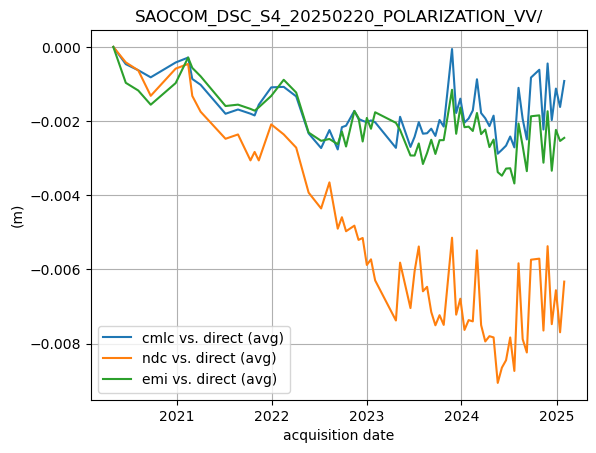
\includegraphics[width=0.8\linewidth]{Figures/mlc/DSC_S4/bias_mem_0.95_past_1.0_ma_0.0_mini_10.png}
    \caption{Deformation bias over time w.r.t. direct interferogram for different phase estimators.}
    \label{fig:bias_direct}
\end{figure}

We are going to analyze the evolution of the phase (or deformation) bias over time. The plot in Fig.~\ref{fig:bias_direct} shows the average displacement difference with respect to the direct interferogram, for points which have a coherence between 0.2 and 0.6 in the direct interferogram. The behavior of PIPE and EMI is very similar. Removing the drift control, i.e. the reference phase calibration step in the PIPE algorithm, introduces a drift of a couple of mm per year. EMI and PIPE exhibit some initial drift too, but this is smaller. The displacement error should become stable in the presence of long-term coherence.

All estimators are affected by a seasonal oscillation, which is likely related to vegetation or soil moisture content.

This analysis is limited by the need for a residual coherence in the direct interferogram. This might explain why the drift seems to stop after 4-5 years.

For this reason, we are also examining the evolution bias with respect to the EMI results. We are going to accumulate the differences at each time step and filter with the short-term coherence as estimated by the PIPE algorithm: this way, targets which are incoherent in the long run are not excluded as in the previous analysis. The plots reported in Fig.~\ref{fig:bias_emi} show that without drift control the drift is about 10 mm / year, whereas for our algorithm the drift appears to stop after reaching an initial value of around 5 mm. Some improvements could limit this initial bias accumulation, which is likely a warm-up effect.

\begin{figure}[htb!]
    \centering
    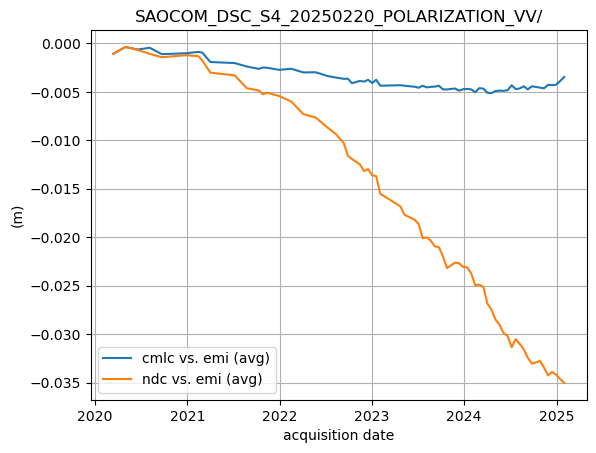
\includegraphics[width=0.8\linewidth]{Figures/mlc/DSC_S4/s1_mem_0.95_past_1.0_ma_0.0_mini_10.png}
    \caption{Deformation bias over time w.r.t. EMI interferogram for different phase estimators, reconstructed from lag-1 interferograms.}
    \label{fig:bias_emi}
\end{figure}


\subsubsection{Analysis of phase standard deviation over time}
The same analysis can be repeated for the standard deviation: the results are reported in Fig.~\ref{fig:std_direct}. In this case, the performance of EMI and PIPE is different. For short temporal intervals, PIPE has a smaller deviation; after two to three years, they are both very similar.

\begin{figure}[htb!]
    \centering
    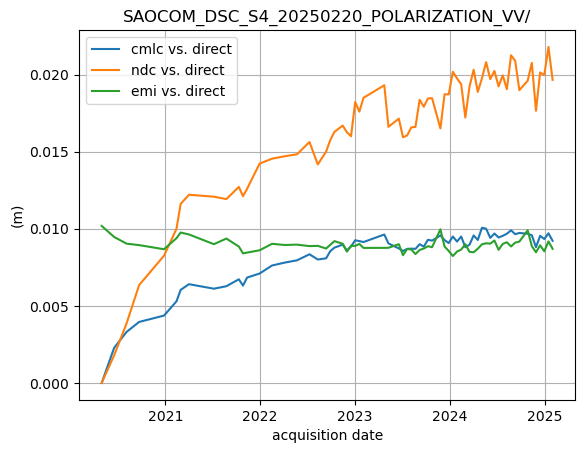
\includegraphics[width=0.8\linewidth]{Figures/mlc/DSC_S4/std_mem_0.95_past_1.0_ma_0.0_mini_10.png}
    \caption{Deformation standard deviation over time w.r.t. direct interferogram for different phase estimators.}
    \label{fig:std_direct}
\end{figure}


%\hl{Do we want to also add the performance having the reference in the middle of the stack?}


\subsection{Relative performance assessment (Sentinel-1)}
This section reports the results of the same analysis applied to the Sentinel-1 case.


\subsubsection{Analysis of phase bias over time}
Figure~\ref{fig:bias_direct_S1} and ~\ref{fig:bias_emi_S1} show the bias over time for a Sentinel-1 case (dataset 124) both w.r.t. the direct interferograms and w.r.t EMI. The observed behaviour is roughly similar but C-band appears to be more susceptible to bias even if the total period is much smaller.

\begin{figure}[ht!]
    \centering
    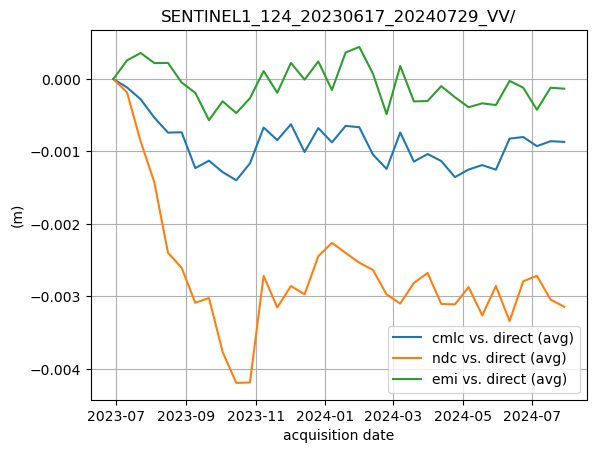
\includegraphics[width=0.8\linewidth]{Figures/mlc/S1_124/S1_124_bias_0.98_1.0_0.0.png}
    \caption{Deformation bias over time w.r.t. direct interferogram for different phase estimators.}
    \label{fig:bias_direct_S1}
\end{figure}

\begin{figure}[htb!]
    \centering
    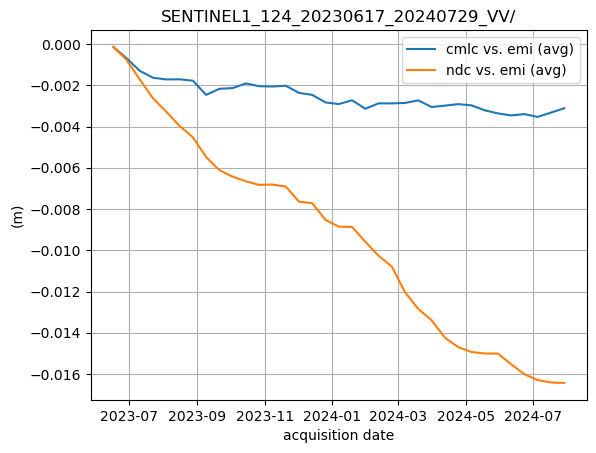
\includegraphics[width=0.8\linewidth]{Figures/mlc/S1_124/S1_124_s1_bias_0.98_1.0_0.0.png}
    \caption{Deformation bias over time w.r.t. EMI interferogram for different phase estimators, reconstructed from lag-1 interferograms.}
    \label{fig:bias_emi_S1}
\end{figure}


\subsubsection{Analysis of phase standard deviation over time}
A similar conclusion holds also for the standard deviation measured w.r.t. the direct interferogram (see Fig.~\ref{fig:std_direct_S1}): the behavior is similar between C and L-band, but the discrepancy between the proposed algorithm and EMI is a bit larger. This might have to do with the choice of parameters for the processing (e.g. the auto-regressive coefficient for the running reference).

\begin{figure}[htb!]
    \centering
    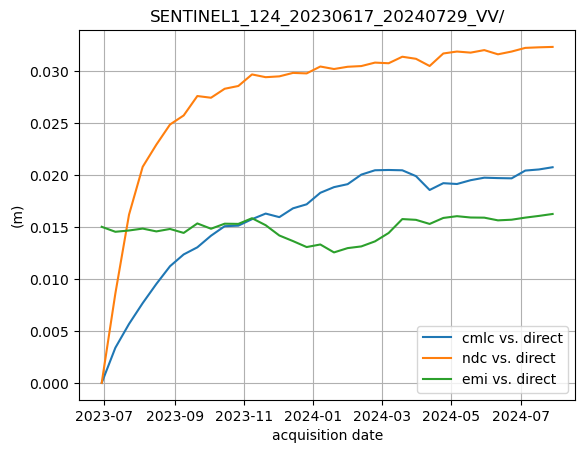
\includegraphics[width=0.8\linewidth]{Figures/mlc/S1_124/S1_124_std_0.98_1.0_0.0.png}
    \caption{Deformation standard deviation over time w.r.t. direct interferogram for different phase estimators.}
    \label{fig:std_direct_S1}
\end{figure}







\subsection{Theoretical models}
\label{sec:cmlc_models}
To assess the performance in an absolute sense, we resort to simulated data for which we know the desired output phase. 

We model the coherence over time as a stationary process with the following function of time:
\begin{equation}
    \gamma(t) = \gamma_1 e^{-|t|/t_1 -j \omega_1 t } + \gamma_2 e^{-|t|/t_2 -j \omega_2 t } + \gamma_3 e^{-|t|/t_3 -j \omega_3 t },
\end{equation}
for  $t \neq 0$ (and $\gamma(0)=1$), with the following values for the parameters:
\begin{equation}
    \begin{matrix}
    \gamma_1 = 0.18 &   t_1 = 11 \, \mathrm{days} &  \omega_1 = 0.030 \, \mathrm{rad/day}\\
    \gamma_2 = 0.25& t_2 = 50 \, \mathrm{days} & \omega_2 = 0.002  \, \mathrm{rad/day}\\
    \gamma_3 = 0.13 &  t_3 = \infty \, \mathrm{days} & \omega_3 = 0.000  \, \mathrm{rad/day} \\
    \end{matrix} 
    \nonumber
\end{equation}
This parametrization ensures the presence of non-zero closure phases, which have the potential to generate a bias in the estimated phases and thus deformation drifts, especially when integrating short-term multilooked phases. The first two terms represent targets which are both decorrelating and rotating, f.i. because of an accumulation of biomass; the third target is not decorrelating. Values are taken from a previous study of Sentinel-1 data. A precise correspondence to reality is anyway not crucial for the verification of the algorithm.

We then performed 1000 Monte-Carlo simulations for 8 years of acquisitions with a repeat pass of 16 days and according to the coherence model described above. For each acquisition, we generated 200 independent samples (looks). Finally, we applied both the EMI and PIPE estimators to the synthetic data.

Figure~\ref{fig:bias_synth} shows the phase bias as a function of time for both estimators. The EMI results show a very small bias, which confirms that EMI is a good estimator provided that there is a long-term coherence contribution.
The PIPE results show an initial bias build-up but, after 1-2 years, there is no permanent drift in the estimated deformation.

\begin{figure}[htb!]
    \centering
    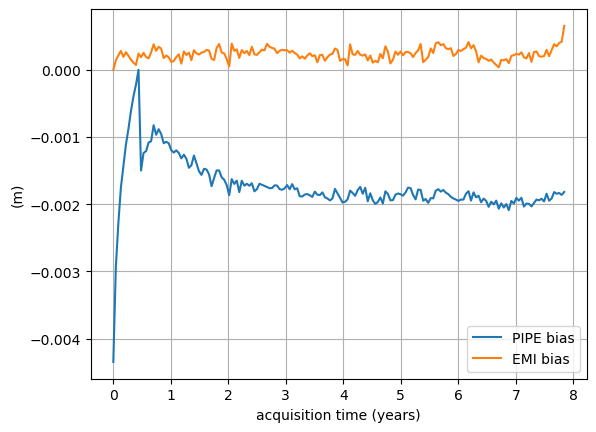
\includegraphics[width=0.48\linewidth]{Figures/mlc/PIPE_Synthetic/PIPE_bias_EMI_bias.png}
    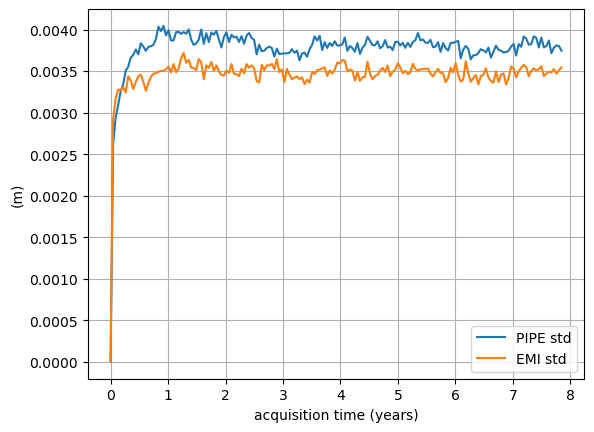
\includegraphics[width=0.48\linewidth]{Figures/mlc/PIPE_Synthetic/PIPE_std_EMI_std.png}
    \caption{Deformation bias (left) and standard deviation (right) over time for EMI and PIPE phase estimators.}
    \label{fig:bias_synth}
\end{figure}


\subsubsection{Internal coherence modelling}
The PIPE algorithm computes two important interferograms: one is the interferogram between the running reference and the new incoming acquisition (which is the basis for the phase product itself); the other is the interferogram between the running reference and a past reference, which is necessary to keep the phase drift under control (see Fig.~\ref{fig:internal_coherence_cartoon}). Knowing the ``true'' coherence between any two acquisitions makes it possible to predict those two coherence values, which we can then compare with the observed values to verify the internal working of the algorithm.

\begin{figure}[htb!]
    \centering
    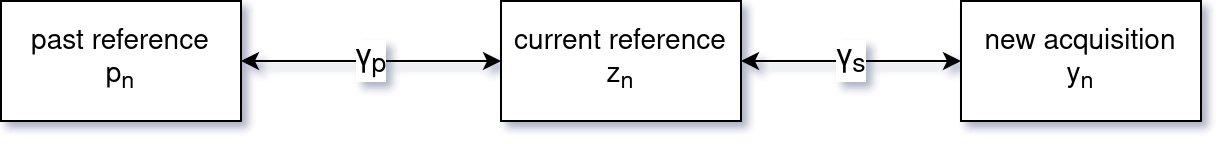
\includegraphics[width=0.8\linewidth]{Figures/mlc/PIPE_Synthetic/Two_coherences.drawio.png}
    \caption{Two coherence values are computed inside the PIPE algorithm, one is the short-term coherence between the running reference and the incoming acquisition, the other is between the running reference and the past reference to calibrate the phase of the running reference.}
    \label{fig:internal_coherence_cartoon}
\end{figure}

Both past and running references are really just linear combinations of the original acquisitions. Knowing the weights from the parameters chosen for the PIPE algorithm, and assuming perfect phase reconstruction, we can derive the said coherence. In general, if $y'$ and $y''$ are two linear combinations of the original acquisitions $y_i$, such as:
\begin{align}
y' &= \sum_i w_i' \, y_i \\
y'' &= \sum_i w_i''\,  y_i, \\
\end{align}
the correlation is
\begin{equation}
    \mathrm{corr}(y', y'')= \sum_{i,j} w_i' w_j'' \, \gamma(y_i, y_j).
\end{equation}
Finally, the coherence is going to be:
\begin{equation}
    \gamma(y', y'') = \frac{\mathrm{corr}(y', y'')}{\sqrt{\mathrm{corr}(y', y') \ \mathrm{corr}(y'', y'')}}.
\end{equation}
In particular, the running reference $z_{n+1}$ can be written explicitly (and approximately) as
\begin{equation}
    z_{n+1} = y_n + \alpha\,y_{n-1} + \alpha^2\,y_{n-2} + \cdots,
    \label{eqn:running_linear}
\end{equation}
and therefore $1, \, \alpha, \, \alpha^2\, \cdots$ are the weights to be considered in the equations above.

Figure~\ref{fig:internal_coherence} shows the evolution of the coherence for the two interferograms, which are computed inside the PIPE algorithm and the theoretical values derived from the formulas described here. After an initial transition, which we have not modeled, it appears that the coherence settles close to the expected values, confirming the inner workings of the algorithm.

\begin{figure}[htb!]
    \centering
    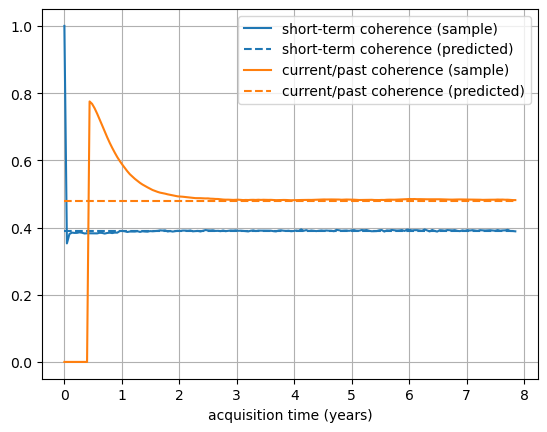
\includegraphics[width=0.8\linewidth]{Figures/mlc/PIPE_Synthetic/coherences_predicted_vs_sampled.png}
    \caption{Predicted vs. sampled coherence for the two internal interferograms computed in the PIPE algorithm.}
    \label{fig:internal_coherence}
\end{figure}

The ultimate goal of this analysis was to derive the standard deviation of the estimated phase from the coherence levels. Unfortunately, the results do not show a level of match with the simulations sufficient for this kind of theoretical analysis. In the analysis, we have not modeled the uncertainty in the phases that enter the linear combination of the acquisition (e.g. in Eq.~\ref{eqn:running_linear} ). It seems that this kind of approximation is sufficient to estimate properly the average coherence (where the error intervenes as a second order term) but not the phase uncertainty itself (where the error intervenes directly). Further attempts in this direction were not sufficient for a satisfactory theoretical modeling.

\subsection{Computational performance}
\label{sec:cmlc_computation}

The computational performance of the phase-estimation algorithm proposed here is very high (i.e. the algorithm is very efficient). The cost is only a few complex multiplications for each pixel, and for each new incoming acquisition. A full-covariance matrix approach would have a cost that grows quadratically with the number of acquisitions and would require the simultaneous access to the entire acquisition history, at least for the multi-looking window.

At the moment it looks like the most expensive step is the geocoding from \acs{cmlc} to \acs{gmlc}. This cost is comparable to the one for generating \acs{nrb} products but could be reduced by adopting a simpler geocoding strategy.

\subsection{Criticalities and weakness}
\label{sec:cmlc_criticalities}

The performance study has shown that there is a needed warm-up period in which the phase is drifting. If this is not acceptable, it is necessary to delay the delivery of the product so that the bias can be corrected, for example, with the application of a full-covariance matrix estimator.

The sampling of the phase signal is not optimal as it is performed in the demonstration software. Since the final product should be sampled on a 50 m grid, the underlying multi-looking should be performed on an area larger than $(50 \mathrm{m})^2$. Otherwise, there is a risk of frequency aliasing (actually, this is not limited to phase products).

After that, resampling to UTM grid should pose no major problem since the signal is already properly sampled at the \acs{cmlc} level.